\documentclass[UTF8]{ctexart} 
\usepackage{amsmath} 
\usepackage{graphicx}
\usepackage{pythonhighlight}
\usepackage{indentfirst}
\usepackage{amsfonts}
\begin{document} 

\title{Homework 2}
\author{Ji Jiabao}
\maketitle

\subsection*{Exer.1:}
    First, consider taking $n - 2$ comparisons.
    If we list the $n - 2$ comparisons like below, and we get the maximal $M$ from them.
    $$
        a_{i_1} \leq a_{j_1},
        a_{i_2} \leq a_{j_2},
        \dots
        a_{i_{n -2}} \leq a_{j_{n - 2}}
    $$

    For smaller array $a_{i_1}, a_{i_2}, ... a_{i_{n - 2}}$, there are at most $n - 2$ different element from
    the original array. Choose 2 in the others as $a_{x}, a_{y}$, at least one of them is not maximal,
    suppose $a_{x}$ is not maximal, then if we change $a_x$ to $a_{x} = M + 1$, the new array still suffices 
    the $n - 2$ comparisons, but the maximal is not $M$ anymore.

    Next, if we take $m < n - 2$ comparisons, the proof is similar to the case above. The smaller array
    has at most $m$ different elements, and at least $n - m$ element are not in the smaller part, we can still
    choose one from them not maximal, and change it to maximal + 1, leading to the parodox.


\subsection*{Exer.2:}
\begin{python}
    def ComputeMaxMin(A):
        # A is an array with n = 2m elements
        n = len(A)
        m = n // 2
        MinCandidate = []
        MaxCandidate = []
        for i in range(m):
            x = A[2 * i]
            y = A[2 * i + 1]
            if (x < y):
                MinCandidate.append(x)
                MaxCandidate.append(y)
            else:
                MinCandidate.append(y)
                MaxCandidate.append(x)
        
        Min = sys.maxint
        Max = -sys.maxint
        for i in range(m):
            if MinCandidate[i] < Min:
                Min = MinCandidate[i]
            if MaxCandidate[i] > Max:
                Max = MaxCandidate[i]
        return Min, Max
\end{python}
    \hspace*{1em} Based on the algorithm above, we can get the minimal element and maximal element in the $n$ items
    with exactly $\frac{3}{2} n - 2$ comparisons.

    Since the array has $n = 2m$ elements, we can first compare any consecutive two elements in the array    for $m$ times to divide the original array into two subarray as $MaxCandidate$, $MinCandidate$. We know for sure that
    maximal element is in $MaxCandidate$ and minimal element is in $MinCandidate$.
    
    Using the result in  $Exer.1$, we need $m - 1$ times of comparisons to get minimal element form $MinCandidate$
    and another $m - 1$ comparisons for maximal. In all, we do $m + m - 1 + m - 1 = 3m-2 =\frac{3}{2}n - 2$ comparisons.

\subsection*{Exer.3:}
\begin{python}
class Node:
    def __init__(self, weight, father, biggerSon, smallerSon):
        self.weight = weight
        self.father = father
        self.biggerSon = biggerSon
        self.smallerSon = smallerSon

def ComputeSecondMax(A):
        # A should be an array with 2^k elements
        comparisons = 0
        n = len(A)
        k = math.floor(math.log(n, 2))
        MaxCandidate = []
        for x in A:
            MaxCandidate.append(Node(x, None, None, None))
        for _ in range(k):
            tmpMaxCandidate = []
            for j in range(len(MaxCandidate) // 2):
                x = MaxCandidate[2 * j]
                y = MaxCandidate[2 * j + 1]
                if (x.weight < y.weight):
                    comparisons += 1
                    newNode = Node(y.weight, None, y, x)
                    tmpMaxCandidate.append(newNode)
                    x.father = newNode
                    y.father = newNode
                else:
                    comparisons += 1
                    newNode = Node(x.weight, None, x, y)
                    tmpMaxCandidate.append(newNode)
                    x.father = newNode
                    y.father = newNode
            MaxCandidate = tmpMaxCandidate

        res = 0
        curNode = MaxCandidate[0]
        for _ in range(k):
            if curNode.smallerSon.weight > res :
                res = curNode.smallerSon.weight
                comparisons += 1
            comparisons += 1
            curNode = curNode.biggerSon
        return comparisons, res
\end{python}
    \hspace*{1em} The algorithm is similar to the one in $Exer.2$, we can divide the original array for $k$ times, each time, we 
    get the bigger element from consecutive 2 elements in the last iteration. The array size is $2^k, 2^{k - 1}...2^{1}$
    And it takes $2^{i - 1}$ comparisons for $2^i$ size array. But to get the second max element we still need to do something else.
    \begin{figure}[h]
        \centering
        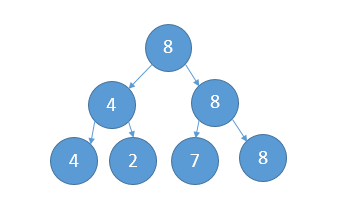
\includegraphics[]{2-wayTree.png}
        \caption{Comparing Tree in Exer.3}
    \end{figure}
    \hspace*{1em}After $k$ iterations of comparing consecutive elements, we constructed the comparing tree above.
    Obviously, the maximal element floats up from bottom to top, and the candidates for second maximal element
    are those who once compared to the maximal element in the tree, 4 and 7 in below specific tree, for example.\\
    \hspace*{1em}So we need to compare another $log_2(n) - 1$ times to get the maximal element in the candidates since maximal element 
    needs to be compared for $log_2(n)$ times to float to top.\\
    \hspace*{1em}In all we do $1 + 2 + 2^2 +... + 2^{k - 1} + log_2(n) = n + log_2(n)$ comparisons.\\

\subsection*{Exer.4:}
    From the sum equation in the class, we can derive the result as follows.
\begin{align*}
    \mathbb{E}  & = \sum_{i \neq j} \frac{1}{|i - j| + 1}\\
                & = 2\sum_{1 \leq i < j \leq n} \frac{1}{j - i + 1}\\
                & = 2(\frac{1}{1 + 1}(n - 1) + \frac{1}{2 + 1}(n - 2) + ... + \frac{1}{n - 1 + 1}(n - (n - 1)))\\
                & = 2(\frac{1}{2}n + \frac{n}{3} + ... + \frac{n}{n} - (\frac{1}{2} + \frac{2}{3} + ... + \frac{n - 1}{n}))\\
                & = 2(n(\frac{1}{2} + ... + \frac{1}{n}) - (1 - \frac{1}{2}) - (1 - \frac{1}{3}) -... - (1 - \frac{1}{n}))\\
                & = 2(n(H_n - 1) - (n - 1) + (H_n -1))\\
                & = 2((n + 1)H_n - 2n)\\
                & = 2nH_n + 2H_n - 4n
\end{align*}

\end{document}
